% ****** Start of file langevin.tex ******
%%
\documentclass[%
 reprint,
%superscriptaddress,
%groupedaddress,
%unsortedaddress,
%runinaddress,
%frontmatterverbose, 
%preprint,
%showpacs,preprintnumbers,
%nofootinbib,
%nobibnotes,
%bibnotes,
 amsmath,amssymb,
 aps,
%pra,
%prb,
%rmp,
%prstab,
%prstper,
%floatfix,
]{revtex4-1}

\usepackage{graphicx}% Include figure files
\usepackage{dcolumn}% Align table columns on decimal point
\usepackage{bm}% bold math
\usepackage{subcaption}
%\usepackage{hyperref}% add hypertext capabilities
%\usepackage[mathlines]{lineno}% Enable numbering of text and display math
%\linenumbers\relax % Commence numbering lines

%\usepackage[showframe,%Uncomment any one of the following lines to test 
%%scale=0.7, marginratio={1:1, 2:3}, ignoreall,% default settings
%%text={7in,10in},centering,
%%margin=1.5in,
%%total={6.5in,8.75in}, top=1.2in, left=0.9in, includefoot,
%%height=10in,a5paper,hmargin={3cm,0.8in},
%]{geometry}

\begin{document}

\preprint{APS/123-QED}

\title{Bayesian Analysis of a Time Trace of a Brownian particle in an harmonic potential}

\author{Helmut H. Strey}
 \affiliation{Biomedical Engineering Department, Stony Brook University.}%Lines break automatically or can be forced with \\

\date{\today}% It is always \today, today,
             %  but any date may be explicitly specified

\begin{abstract}
In many fields, but particularly in single molecule experiments, the experimenter is often faced with the problem of measuring time-traces of limited length.  Here we would like to address the question on how to properly extract information from these trajectories. 
\begin{description}
\item[PACS numbers]
May be entered using the \verb+\pacs{#1}+ command.
\end{description}
\end{abstract}

\pacs{Valid PACS appear here}% PACS, the Physics and Astronomy
                             % Classification Scheme.
%\keywords{Suggested keywords}%Use showkeys class option if keyword
                              %display desired
\maketitle

%\tableofcontents
\onecolumngrid
\section{Introduction}
In many fields, but particularly in single molecule experiments, the experimenter is faced with the problem of obtaining time-traces of limited length.  Since the experimental trajectories are driven by both energy-landscape parameters, such as binding energies/spring constant as well as dynamic parameters such as friction or diffusion constants.  Here we would like to address the question on how to properly extract information from these trajectories.  Specifically, we are interested in probability distributions of model parameters given the measured data.  To address this question, we will investigate a toy problem from statistical physics that is often used in single molecule/particle experiments:�� an overdamped Brownian particle in a harmonic potential with Hook's constant k and friction coefficient $\gamma$.  The Langevin equation for such a system can simply be written by:
\begin{equation}
\dot x =  - \frac{k}{\gamma }x + \frac{1}{\gamma }f(t)
\end{equation}
where k is the spring constant, gamma is the friction coefficient and f(t) is a randomly fluctuating force.  The solution to this Langevin equation is given by:
\begin{equation}
\left\langle {x(0)x(t)} \right\rangle  = \frac{{k_B}T}{k} \exp \left( { - \frac{k}{\gamma }t} \right)
\end{equation}
The amplitude of the fluctuation is determined by the equipartition theorem, and the relaxation time is determined by the ratio of friction and spring constant.  For convenience, let us rewrite eq.2 using the mean-square-amplitude $\sigma^{2}=\langle {x^2} \rangle=k_{B}T/k$ and the relation time $\tau=\gamma/k$:
\begin{equation}
\left\langle {x(0)x(t)} \right\rangle  = \sigma^{2} \exp \left( {- \frac{t}{\tau}} \right)
\end{equation}
Us and others have analyzed such time trajectories by calculating the autocorrelation function and then fitting it to an exponential function to extract the spring constant k and the friction coefficient gamma by a least square fit.  In this paper we will show that this procedure can become misleading when performed over short time sequences on the order of several relaxation times even when these fits are performed on autocorrelation averages over several time trajectories.  To fully extract the information from individual and sets of trajectories we employ a Bayesian analysis on the time trace that is based on the likelihood function of a time trace of a particle in a harmonic oscillator.  To illustrate the strength of the method, we simulate short time trajectories of several relaxation times and estimate the posterior probability distributions for the model parameter using modern Markov chain Monte Carlo (MCMC) methods.  We will also compare those results with analytic estimates.
\section{Autocorrelation function Analysis}
\begin{figure}
  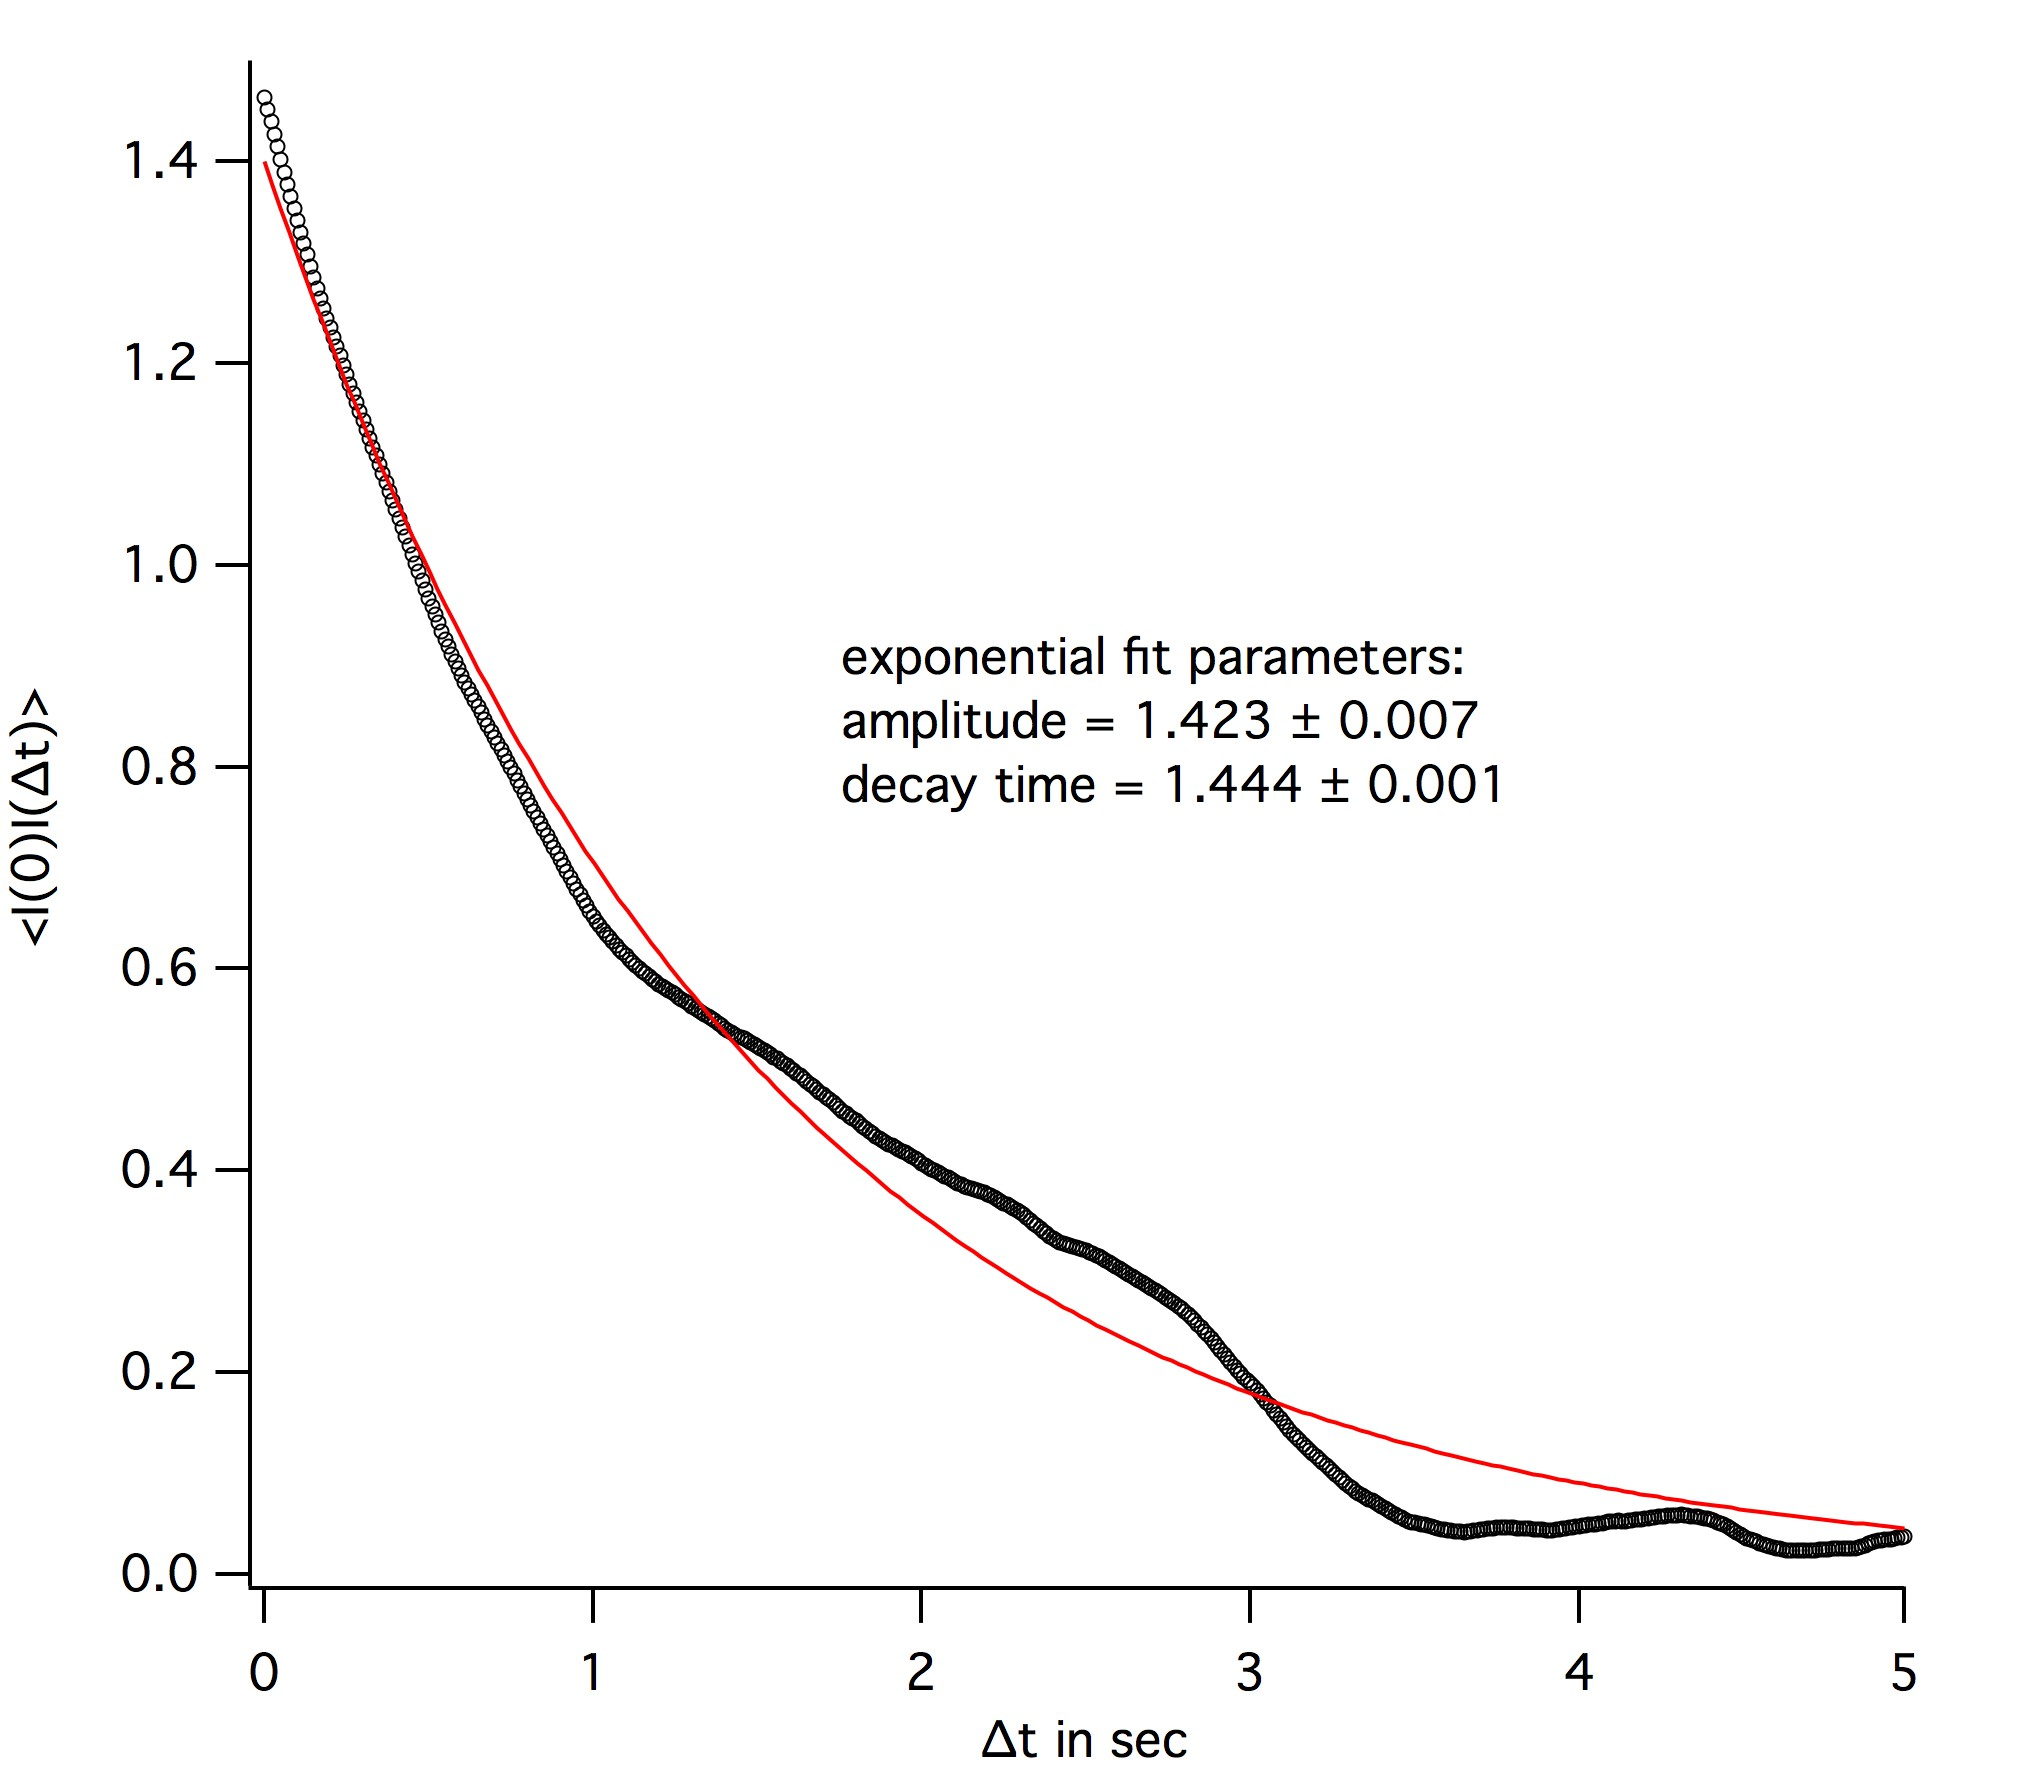
\includegraphics[width=0.5\linewidth]{acf10000.jpg}
  \caption{Autocorrelation function of a simulated particle in a harmonic potential with parameters: $\sigma^{2}=\langle {x^2} \rangle = 1$ and $\tau=1$. The non-linear least square fit to the data used the Levenberg-Marquart algorithm.}
  \label{fig:acf10000}
\end{figure}
To illustrate the problem with analyzing auto-correlation functions (acf), we simulated 10,000 points of an overdamped particle in a harmonic oscillator using the conditional probabilities from eq.4.  The parameters for the simulation were $\sigma^{2}=\langle {x^2} \rangle = 1$, $\tau=1$, and $\Delta t=0.01 sec$.
We calculated the correlation function by Fast Fourier Transformation (cite Numerical Recipies).  Fig. 1 shows the decaying acf and the non-linear least-square fit to a decaying exponential function.  This particular fit resulted in an amplitude of $\sigma^{2}=1.423\pm0.007$ and a decay time of $\tau=1.444\pm0.001$.  Both parameters are reasonable given that we only analyzed over 100 decay times, but the standard deviation of the parameters is extremely optimistic: the amplitude is off by 60 standard deviations and the decay time is off by 444!
From a visual inspection it is also clear that the residuals are highly correlated in time which is not surprising given that the acf was calculated from a continuous time series.  What is concering to us is that in many publications the parameters of a least-square fit to a correlation function are taken at face value including their estimated confidence intervals.  To get a better sense for the distributions of the parameters we simulated 10,000 time series of 10,000 points each and plotted histogramms of each of the parameters in Fig.2.  Over these samples, the amplitude has a mean of $1.04$ and a standard deviation of $0.52$ whereas the decay time has an average of $1.29\pm1.70$.  This distribution paints a very different picture.  The amplitude has a $50\%$ uncertainty and the decay time is uncertain by more than $100\%$.  To see which estimate of the uncertainty is correct, let us attempt to estimate the error.  The uncertainty of the amplitude should be given by how many independent measures we can expect.  Since we simulated 100 times the decay time we estimate that we should expect 100 independent measures of $\sigma^{2}$ and therefore the uncertainty of the amplitude should be the square root of that or around $10\%$.  The estimate of the decay time is not as easy, but we can estimate how accurately we can measure $\tau$ by considering that since $\Delta t$ is small each time point is an independent measure, resulting in a $1\%$ uncertaintly for $\tau$. We will now see whether a Bayesian Analysis can do better.
\begin{figure}
    \centering
    \begin{subfigure}[b]{0.4\textwidth}
        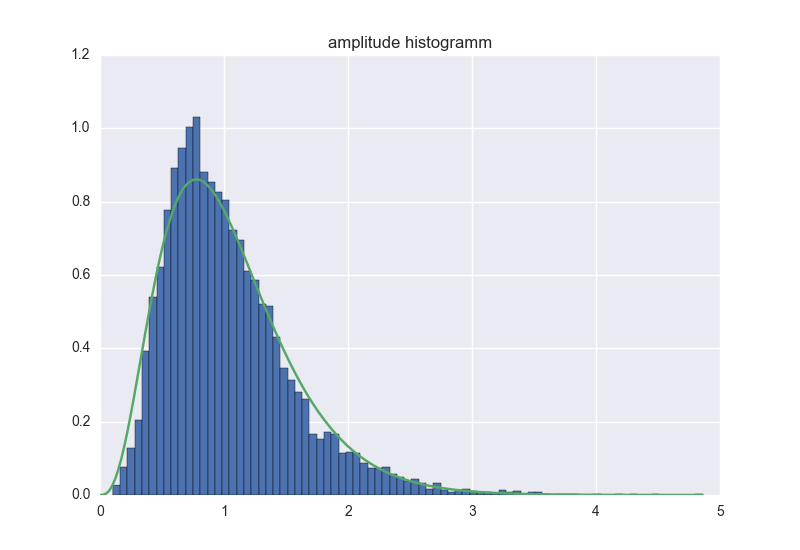
\includegraphics[width=\textwidth]{histA.png}
        \caption{histogram of $\sigma^{2}$}
        \label{fig:histA}
    \end{subfigure}
    ~ %add desired spacing between images, e. g. ~, \quad, \qquad, \hfill etc. 
      %(or a blank line to force the subfigure onto a new line)
    \begin{subfigure}[b]{0.4\textwidth}
        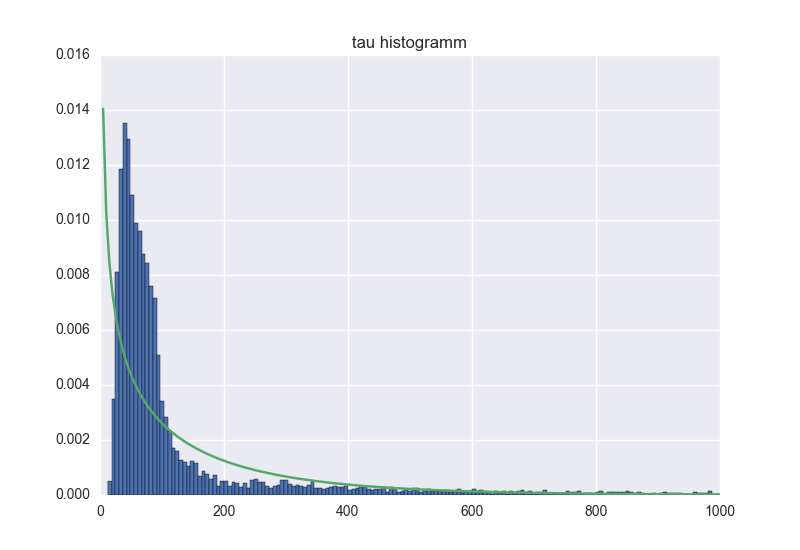
\includegraphics[width=\textwidth]{histtau.png}
        \caption{histogram of decay time $\tau$}
        \label{fig:histtau}
    \end{subfigure}
    \caption{Histograms of non-linear least-square fit parameters of 10,000 time traces of 10,000 points each}\label{fig:hist}
\end{figure}

\section{Bayesian Analysis}
Let us first review the likelihood function and the Bayes theorem.
The likelihood function describes the probability that a particular trajectory $\left\{ {{x_1}({t_1}),{x_2}({t_2}), \ldots ,{x_N}({t_N})} \right\}$ originated from a particular model (eq. 1) with a particular choice of parameters k and gamma.  The likelihood function is the product of the probability of finding $x_0$ at $t_0$ and all the conditional probabilities of finding the particle at $x_{n+1}$ at time $t_{n+1}$ given that they were at $x_n$ at time $t_n$.  Both probabilities are given by the solution of the Smolukowski equation for an overdamped Brownian particle in a harmonic potential.
\begin{equation}
p\left( {x,\Delta t\left| {x_0} \right.} \right) = \frac{1}{{\sqrt {2\pi \sigma^{2}(1-B^{2}(\Delta t))} }}\exp \left( { - \frac{{{{\left( {x - {x_0}B(\Delta t)} \right)}^2}}}{{2\sigma^{2}(1-B^{2}(\Delta t))}}} \right)
\end{equation}
with $B(\Delta t) = \exp \left( { - \frac{D}{A}\Delta t} \right)$.
As expected, at long $\Delta t$ this distribution is a Gaussian with standard deviation $\sigma$.  The corresponding likelihood function for a specific time trace $\left\{x_i(i\Delta t)\right\}$ is:
\begin{equation}
	p\left( \left\{x_i(t_i)\right\} \left| \tau, \sigma^{2} \right.\right) =
	\frac{1}{\sqrt {2 \pi \sigma^{2}} }
	\exp \left( { - \frac{{x_1}^2}{2\sigma^{2}}}\right)
	\frac{1}{{\sqrt {2\pi \sigma^{2}(1-B^{2}(\Delta t))}^{(N-1)} }}
	\exp \left( { - \sum\limits_{i=1}^{N-1}\frac{{{{\left( {x_{i+1} - {x_i}B(\Delta t)} \right)}^2}}}{{2\sigma^{2}(1-B^{2}(\Delta t))}}} \right)
\end{equation}
This is assuming that we do not know anything about the initial state of the oscillator.  Now Bayes theorem tells us that we can reverse the order of the conditional probability to obtain the posterior probability distribution of our model parameters given our data:
\begin{equation}
	p\left( \tau, \sigma^{2}  \left| \left\{x_i(t_i)\right\} \right. \right) = 
	\frac {p\left( \left\{x_i(t_i)\right\} \left| \tau, \sigma^{2} \right.\right)p\left( \tau,\sigma^{2} \right)}
	{p\left( \left\{x_i(t_i)\right\}\right)}
\end{equation}
The second term of the numerator is called the prior and contains all the information about the model parameters before we look at the data.  For example, the fact that $\tau$ and $\sigma^{2}$ are positive is information that we can feed into the prior.  Typically, we will use weakly informative priors so as not to dominate the information that is extracted from the data.  The prior is also a way for us to include information from previous data analysis.  For example, if we have many short traces of data, we could use the posterior of the previous analysis as the prior for the next trace.  In the following we will determine the maximum of the likelihood function and its width as a function of the model parameters.  This allows us to determine the "best" (or most likely) model parameters and their corresponding uncertainties.
\section{Maximum Likelihood}
In this section we will express the likelihood in terms of $\sigma^{2}$ and $B$.  We will also assume uniform priors for both $B$ and $\sigma$.  Later we will explore more appropriate choices for priors.
\begin{equation}
	p\left( \left\{x_i(t_i)\right\} \left| B, \sigma^{2} \right.\right) =
	\frac{1}{\sqrt {2 \pi \sigma^{2}}^{N} }
	\frac{1}{{\sqrt {(1-B^{2})}^{(N-1)} }}
	\exp \left( -\frac{1}{2\sigma^{2}}\left({ {x_1}^{2} + \sum\limits_{i=1}^{N-1}\frac{{{{ {x_{i+1}^{2} - 2x_{i+1}{x_i}B} +{x_i}^{2}B^{2} }}}}{{(1-B^{2})}}} \right)\right)
\end{equation}
In oder to find the maximum likelihood it is convenient to take the logarithm of $p$ and then take the derivatives with respect to $\sigma$ and $B$.
\begin{equation}
\begin{aligned}
	\Phi &= ln \left( p\left( \left\{x_i(t_i)\right\} \left| B, \sigma^{2} \right.\right) \right)\\\\
	&= C - N ln(\sigma) - \frac{N-1}{2}ln \left( 1-B^{2}\right) -\frac{1}{2\sigma^{2}}Q(B)\\
	with \quad Q(B) &= {x_1}^{2} + \sum\limits_{i=1}^{N-1}\frac{ {x_{i+1}^{2} - 2x_{i+1}{x_i}B} +{x_i}^{2}B^{2} }{(1-B^{2})}\\
	&= \frac{x_{1}^{2}+x_{N}^{2}}{1-B^2}+\frac{1+B^2}{1-B^2}\sum\limits_{i=2}^{N-1}x_{i}^{2}-\frac{2B}{1-B^2}\sum\limits_{i=1}^{N-1}x_{i}x_{i+1}
\end{aligned}
\end{equation}
where the fundamental statistic is given by
\begin{equation}
	\begin{aligned}
		a_{EndPoints}&=a_{EP}=x_{1}^{2}+x_{N}^{2}\\
		a_{SumSquared}&=a_{SS}=\sum\limits_{i=2}^{N-1}x_{i}^{2}\\
		a_{Correlation}&=a_{C}=\sum\limits_{i=1}^{N-1}x_{i}x_{i+1}\\
	\end{aligned}
\end{equation}
The derivative with respect to $\sigma$ determines $\sigma_{max}$:
\begin{equation}\label{partialsigma}
	\begin{aligned}
	\frac{\partial}{\partial\sigma}\Phi &= -\frac{N}{\sigma_{max}} +\frac{1}{\sigma_{max}^{3}}Q(B)=0\\
	\sigma_{max}^{2} &= \frac{Q(B_{max})}{N}
	\end{aligned}
\end{equation}
Similarly, we can derive an equation to determine $B_{max}$:
\begin{equation}
	\begin{aligned}
	\frac{\partial}{\partial B}\Phi &= \frac{(N-1)B}{1-B^{2}} -\frac{1}{2\sigma^{2}}\frac{\partial}{\partial B}Q(B)\\
	\frac{\partial}{\partial B}Q(B) &= \sum\limits_{i=1}^{N-1}\frac{ (1-B^{2})(2B{x_i}^{2}- 2x_{i+1}{x_i})+2B({x_{i+1}^{2} - 2x_{i+1}{x_i}B} +{x_i}^{2}B^{2}) }{{(1-B^{2})^{2}}}\\
	&= \sum\limits_{i=1}^{N-1}\frac{ 2B{x_i}^{2} +2Bx_{i+1}^{2} - 2(B^{2}+1)x_{i+1}{x_i}}{{(1-B^{2})^{2}}}
	\end{aligned}
\end{equation}
thus by using eq \ref{partialsigma},
\begin{equation}\label{partialB}
	\begin{aligned}
	\frac{(N-1)B_{max}}{1-B_{max}^{2}} -\left.\frac{1}{2\sigma_{max}^{2}}\frac{\partial}{\partial B}Q(B)\right|_{B_{max}}&=0\\
	\frac{Q(B_{max})}{N}\frac{(N-1)B_{max}}{1-B_{max}^{2}} -\left.\frac{1}{2}\frac{\partial}{\partial B}Q(B)\right|_{B_{max}}&=0
	\end{aligned}
\end{equation}
after collecting the terms we can solve for $B_{max}$
\begin{equation}\label{Bmax2}
	-B_{max}a_{EP}
	+(B_{max}^{3}(N-1)-B_{max}(N+1))a_{SS}
	+(B_{max}^{2}(2-N)+N)a_{C}=0
\end{equation}
The cubic equation in $B_{max}$ has one real root in the $[0,1]$ interval and two roots outside. $\sigma_{max}^2$ can be calculated by inserting the solution for $B_{max}$ into eq \ref{partialsigma}.

Next, we need to calculate the uncertainties of the maximum likelihood estimates.  For this we need to calculate the second derivative of the log-likelihood.
\begin{equation}\label{partialsigmasecond}
	\left.\frac{\partial^2}{\partial\sigma^2}\Phi\right|_{\sigma_{max},B_{max}} = \frac{N}{\sigma_{max}^2} -\frac{3}{\sigma_{max}^{4}}Q(B_{max})
	= -\frac{2N}{\sigma_{max}^{2}}
\end{equation}
\begin{equation}
	\begin{gathered}
	\left.{\frac{\partial^{2}}{\partial B^2}}\Phi\right|_{\sigma_{max},B_{max}} = \frac{(N-1)(1+B_{max}^{2})}{(1-B_{max}^{2})^2} -\left.\frac{1}{2\sigma_{max}^{2}}\frac{\partial^2}{\partial B^2}Q(B)\right|_{B_{max}}\\
	= \frac{(N-1)(1+B_{max}^{2})}{(1-B_{max}^{2})^2} -\left.\frac{N}{2Q(B_{max})}\frac{\partial^2}{\partial B^2}Q(B)\right|_{B_{max}}\\
	= \frac{-(1+B_{max}^{2}(1+2N))a_{EP}-(2B_{max}^{2}(1+2N)+N+1-B_{max}^{4}(N-1))a_{SS}+2B_{max}(1+B_{max}^{2}+2N)a_{C}}{(1-B_{max}^{2})^{2}(a_{EP}+(1+B_{max}^{2})a_{SS}-2B_{max}a_{C})}
	\end{gathered}
\end{equation}
\begin{equation}
	\left.{\frac{\partial^{2}}{\partial\sigma\partial B}}\Phi\right|_{\sigma_{max},B_{max}} =  \left.\frac{1}{\sigma_{max}^{3}}\frac{\partial}{\partial B}Q(B)\right|_{B_{max}}
	=\frac{(N-1)B_{max}}{2\sigma_{max}(1-B_{max}^{2})}
\end{equation}
Eq \ref{partialsigmasecond} gives the familar result that the uncertainty is inversely proportional to the square-root of $N$.

\section{Appropriate Priors}
This solution currently assumes a constant prior for $\sigma$ and $B$.  To introduce a reasonable prior we will first assume that the prior $p(B,\sigma^{2})=p(B)p(\sigma^{2})$ which means that the prior assumes independence of $B$ and $\sigma^2$.  An appropriate prior for $p(B)$ is a Beta distribution since it covers the interval $[0,1]$.  For example, for small $\Delta t$ it make sense to choose a Beta distribution with $\alpha > 1$ and $\beta = 1$ to reflect the fact that we expect $B$ to be close to $1$.  The natural prior for $\sigma^2$ is the inverse gamma distribution since it is a conjugate prior distribution.
The posterior probability distribution is then represented by:
\begin{equation}
	\begin{aligned}
	p(B,\sigma^{2} \left| \left\{x_i(t_i)\right\} \right. ) 
	&= p(B)p(\sigma^{2})p\left( \left\{x_i(t_i)\right\} \left| B, \sigma^{2} \right.\right)\\
	&= B^{\alpha_{B}-1}(1-B)^{\beta_{B}-1}
	\frac{1}{\sigma^{2(\alpha_{IG}+1)}}\exp \left( -\frac{\beta_{IG}}{\sigma^2}\right)
	\frac{1}{\sqrt {2 \pi \sigma^{2}}^{N} }
	\frac{1}{{\sqrt {(1-B^{2})}^{(N-1)} }}
	\exp \left( -\frac{Q(B)}{2\sigma^{2}}\right)
	\end{aligned}
\end{equation}
where $\alpha_{B}$ and $\beta_{B}$ are the shape parameters of the Beta distribution and $\alpha_{IG}$ and $\beta_{IG}$ for the inverse gamma distribution.
This changes the logarithm of the posterior $\Phi$ to:
\begin{equation}
	\Phi = C +(\alpha_{B}-1)ln(B) + (\beta_{B}-1)ln(B-1) - N ln(\sigma) - \frac{N-1}{2}ln \left( 1-B^{2}\right) -\frac{1}{2\sigma^{2}}Q(B)
\end{equation}
this addition does not change $\sigma_{max}$ (see equation \ref{partialsigma}).  On the other hand, the derivative with respect to B is then:
\begin{equation}\label{partialB2}
	\begin{aligned}
	\frac{\partial}{\partial B}\Phi &= 
	\frac{\alpha-1}{B}+
	\frac{(N-1)B}{1-B^{2}} -\frac{1}{2\sigma^{2}}\frac{\partial}{\partial B}Q(B)\\
&=\frac{(1-B^{2})(\alpha-1)+(N-1)B^{2}}{(1-B^{2})B}-\frac{1}{2\sigma^{2}}\frac{\partial}{\partial B}Q(B)
	\end{aligned}
\end{equation}
again, we can combine eqs \ref{partialsigma} and \ref{partialB2} to calcualte $B_{max}$:
\begin{equation}
	Q(B_{max}) \frac{(1-B^{2})(\alpha-1)+(N-1)B^{2}}{(1-B^{2})B} =
	\frac{N}{2}\frac{\partial}{\partial B}Q(B)\mid_{B_{max}}
\end{equation}
\begin{acknowledgments}
We wish to acknowledge discussions with Ken Dill
\end{acknowledgments}

\end{document}
